
\chapter{实验室坐标系和体固坐标系中的角动量代数}

整本书我们都使用Edmonds\cite{Ed57}对于角动量耦合的约定和术语。唯一我们需要细细探究的地方就是如何把角动量转换到体坐标系。我们应当在Edmonds{[}Ed
57, Chap,IV{]}的意义下做这个转换。

为了研究Hilbert空间中的波函数在坐标系转动下的性质，我们应当首先考虑一个一维的例子
\begin{comment}
明明是二维。
\end{comment}
。

\begin{figure}[h]
\centering{}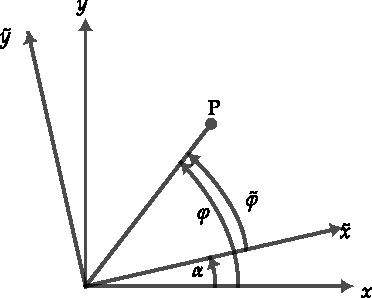
\includegraphics{pictures/绘图}
\end{figure}

令$f(\varphi)$是一个只依赖于相对于体系$z$轴的函数。在体系转动$\alpha$角后，空间中固定一点P对应的角$\varphi$变为角$\tilde{\varphi}=\varphi-\alpha$。因为函数$f$在固定点P的值在坐标系变换下不变，原坐标系中的函数$f$变成了新坐标系中的一个新函数$\tilde{f}$，具有性质：

\begin{equation}
\tilde{f}(\tilde{\varphi})=f(\varphi)=f(\tilde{\varphi}+\alpha)=\mathrm{e}^{\mathrm{i}\alpha J_{z}}f(\tilde{\varphi})
\end{equation}

或者，如果我们改变一下自变量
\begin{comment}
nomenclature不是这么翻译，我根据语境改的。
\end{comment}
，使用$\varphi$而不是$\tilde{\varphi}$，

\begin{equation}
\tilde{f}(\varphi)=\mathrm{e}^{\mathrm{i}\alpha J_{z}}f(\varphi)\quad\text{这里}J_{z}=\frac{1}{\mathrm{i}}\frac{\partial}{\partial\varphi}
\end{equation}

在三维旋转的情况，我们使用在\cite[Chap.I]{Ed57}中定义的Euler角$\Omega=(\alpha,\beta,\gamma)$：在转动了$\Omega$的情况下，波函数$|\Psi\rangle$变为：

\begin{equation}
|\tilde{\Psi}\rangle=R(\Omega)|\Psi\rangle\label{eq:=008F6C=0052A8=004E0B=006CE2=0051FD=006570=007684=0053D8=006362}
\end{equation}

这里酉旋转算符：

\begin{equation}
R(\Omega)=\mathrm{e}^{\mathrm{i}\alpha J_{z}}\mathrm{e}^{\mathrm{i}\beta J_{y}}\mathrm{e}^{\mathrm{i}\gamma J_{z}}
\end{equation}

这里$J_{x},J_{y},J_{z}$作用于坐标系$\boldsymbol{x}_{1},\dots,\boldsymbol{x}_{A}$上。正如在\cite{Ed57}中讨论的，我们也可以引入自旋。$\boldsymbol{J}$就是轨道角动量和自旋角动量的和。

和Hilbert空间中的矢量变换类似，我们可以得到一个算符$T$的变换：

\begin{equation}
T\rightarrow\tilde{T}=RTR^{\dagger}
\end{equation}

根据定义，对于一个球谐张量$T_{\lambda\mu}${[}Ed 57, Eq. (5.2.1){]}我们发现：

\begin{equation}
\tilde{T}_{\lambda\mu}=R(\Omega)T_{\lambda\mu}R^{\dagger}(\Omega)=\sum_{\mu^{\prime}}D^{\lambda}_{\mu^{\prime}\mu}(\Omega)T_{\lambda\mu^{\prime}}
\end{equation}

这里Wigner函数$D^{\lambda}_{\mu^{\prime}\mu}(\Omega)$可以给出：

\begin{equation}
D^{\lambda}_{\mu^{\prime}\mu}(\Omega)=\langle\lambda\mu^{\prime}|R(\Omega)|\lambda\mu\rangle
\end{equation}

我们现在希望研究在特定时间$t$从实验室坐标系到体固坐标系做的转动$\Omega$。记住角动量算符$J_{x},J_{y},J_{z}$是绕$x,y,z$轴无穷小转动的生成元，我们可以把这些算符表示为关于Euler角$\alpha,\beta,\gamma$的微分算符。例如，我们能通过改变Euler角$\alpha$一个$\delta\varphi$的小量而不改变体固坐标系得到绕$z$-轴$\delta\varphi$角的转动，也就是说：

\begin{equation}
L_{z}=-\frac{1}{\mathrm{i}}\frac{\partial}{\partial\alpha}\hat{=}J_{z}
\end{equation}

利用同样的方式，从Euler角的定义\cite{Ed57}中我们得到：

\begin{equation}
-\frac{1}{\mathrm{i}}\frac{\partial}{\partial\beta}\equiv J_{y^{\prime}}=\mathrm{e}^{\mathrm{i}\alpha J_{z}}J_{y}\mathrm{e}^{-\mathrm{i}\alpha J_{z}}=\cos\alpha J_{y}+\sin\alpha J_{x}
\end{equation}

和：

\begin{align}
-\frac{1}{\mathrm{i}}\frac{\partial}{\partial\gamma} & \equiv J_{z^{\prime\prime}}=\mathrm{e}^{\mathrm{i}\alpha J_{z}}\mathrm{e}^{\mathrm{i}\beta J_{y}}J_{z}\mathrm{e}^{-\mathrm{i}\beta J_{y}}\mathrm{e}^{-\mathrm{i}\alpha J_{z}}\nonumber \\
 & =\cos\beta J_{z}-\sin\beta(\cos\alpha J_{x}-\sin\alpha J_{y})
\end{align}

反解得到：

\begin{align}
L_{x} & \equiv\frac{1}{\mathrm{i}}\left(-\cos\alpha\cot\beta\frac{\partial}{\partial\alpha}-\sin\alpha\frac{\partial}{\partial\beta}+\frac{\cos\alpha}{\sin\beta}\frac{\partial}{\partial\gamma}\right)\hat{=}J_{x}\nonumber \\
L_{y} & \equiv\frac{1}{\mathrm{i}}\left(\sin\alpha\cot\beta\frac{\partial}{\partial\alpha}-\cos\alpha\frac{\partial}{\partial\beta}-\frac{\sin\alpha}{\sin\beta}\frac{\partial}{\partial\gamma}\right)\hat{=}J_{y}\\
L_{z} & \equiv\frac{1}{\mathrm{i}}\left(-\frac{\partial}{\partial\alpha}\right)\hat{=}J_{z}\nonumber 
\end{align}
 

它们是角动量
